% ========== SUBSECTION: GANTT CHART ==========
% Symphony: An AI-First Development Environment
% Chapter 2 - Project Planning & Requirements
% Subsection: Gantt Chart

\subsection*{2.0.2 Gantt Chart}
\addcontentsline{toc}{subsection}{2.0.2 Gantt Chart}
\label{subsec:gantt-chart}

It's a type of bar chart used in project management, it illustrates the schedule of the project by showing the duration (start and end dates) of each activity of the project. Each bar of the chart represents an activity where the start of the activity depends on the completion of its prerequisites.

\subsubsection*{Project Timeline Overview}

The compact Gantt chart provides a high-level view of Symphony's development timeline, showing major phases and their durations across the project lifecycle.

\begin{figure}[H]
\centering
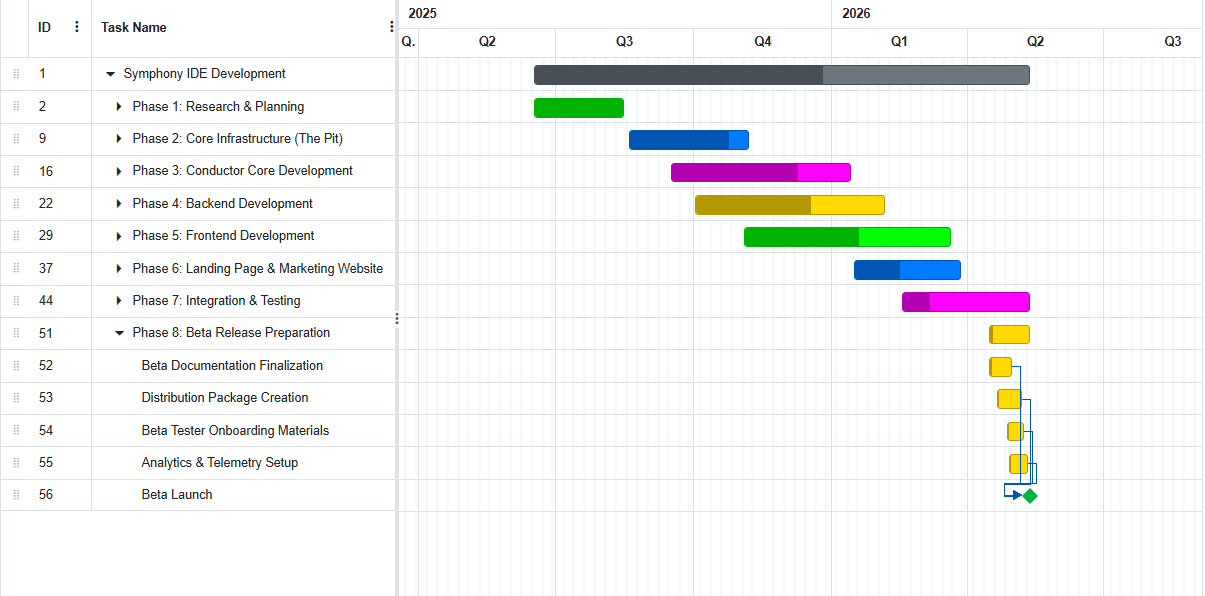
\includegraphics[width=0.95\textwidth]{images/gantt/compact.PNG}
\caption{Symphony Project Timeline - Compact View}
\label{fig:gantt-compact}
\end{figure}

\subsubsection*{Detailed Phase Breakdown - Part 1}

The first detailed view shows the initial development phases including requirements analysis, system design, core infrastructure implementation, and foundation components development with their specific tasks and dependencies.

\begin{figure}[H]
\centering
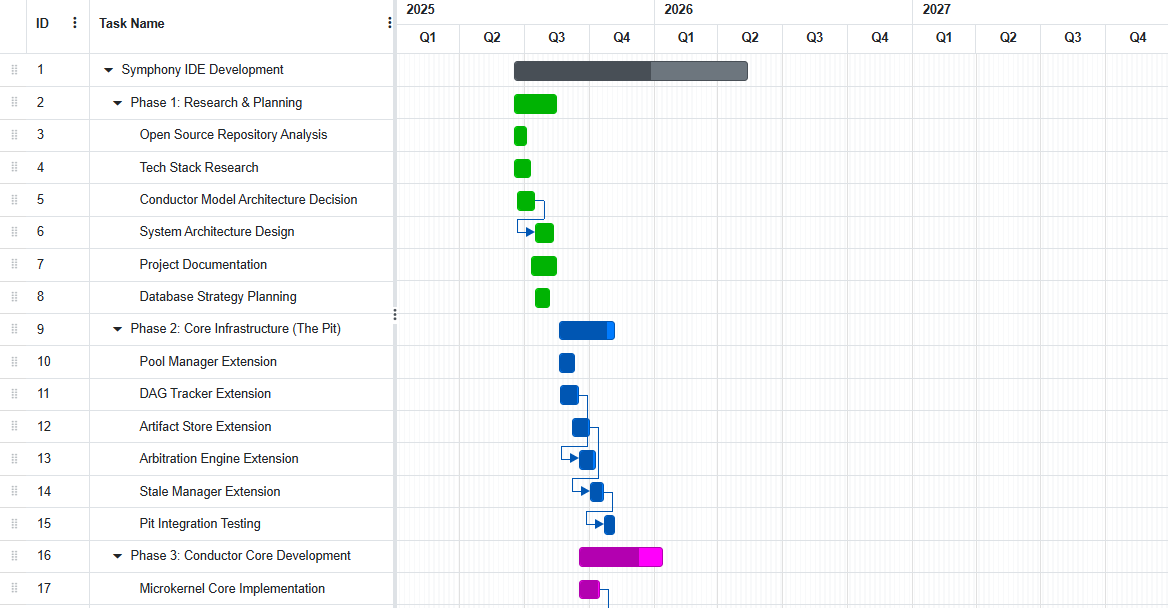
\includegraphics[width=0.95\textwidth]{images/gantt/detailed1.PNG}
\caption{Symphony Project Timeline - Detailed View Part 1}
\label{fig:gantt-detailed1}
\end{figure}

\subsubsection*{Detailed Phase Breakdown - Part 2}

The second detailed view covers the later development phases including extension system implementation, orchestration system development, testing and validation, deployment preparation, and documentation completion.

\begin{figure}[H]
\centering
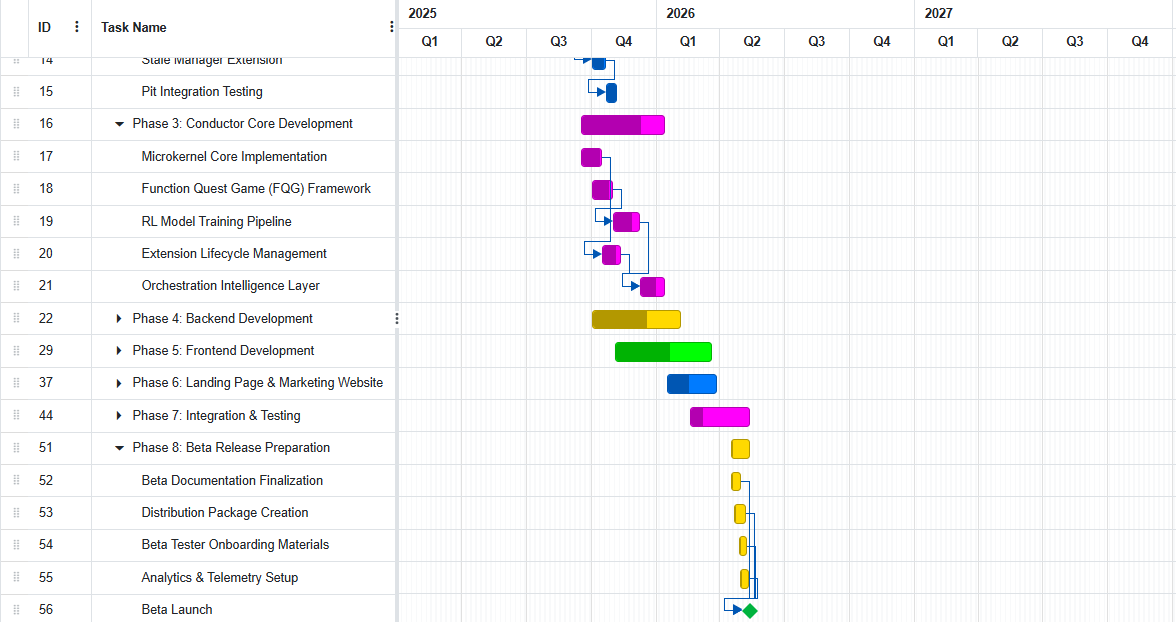
\includegraphics[width=0.95\textwidth]{images/gantt/detailed2.PNG}
\caption{Symphony Project Timeline - Detailed View Part 2}
\label{fig:gantt-detailed2}
\end{figure}